\section{WC 17/3/25}

\subsection*{Overview:}
This week I spent time working on my software. I have improved many 'quality of life' features which make my note taking suite easier and simpler to use day to day

\subsection*{Achievements, Thoughts and Ideas:}
Last week I had planned for this week to be spent fully on my whiteboard note editor however I continued to run up against some challenges in making this functional. I have decided to pause this development on focus on the other necessary features required before my prototype launches. In a couple of weeks (current plan is first week of April - timeline updated to reflect change). By this time I suspect the documentation for the new version of Fabric JS will be more developed resulting in a days worth of work now to understand a feature shortly becoming a few minutes worth.

Instead of my regular scheduled EPQ lesson the main event this week was EPQ day - a day dedicated to working on my project and supporting documentation. An example of my feature additions this week can be seen here: \nameref{prototype:LoadingSpinner}. Please see my full plan for the day here and reflection in what I achieved: \nameref{planning:EPQDayPlan}

\begin{figure}[H]
    \centering
    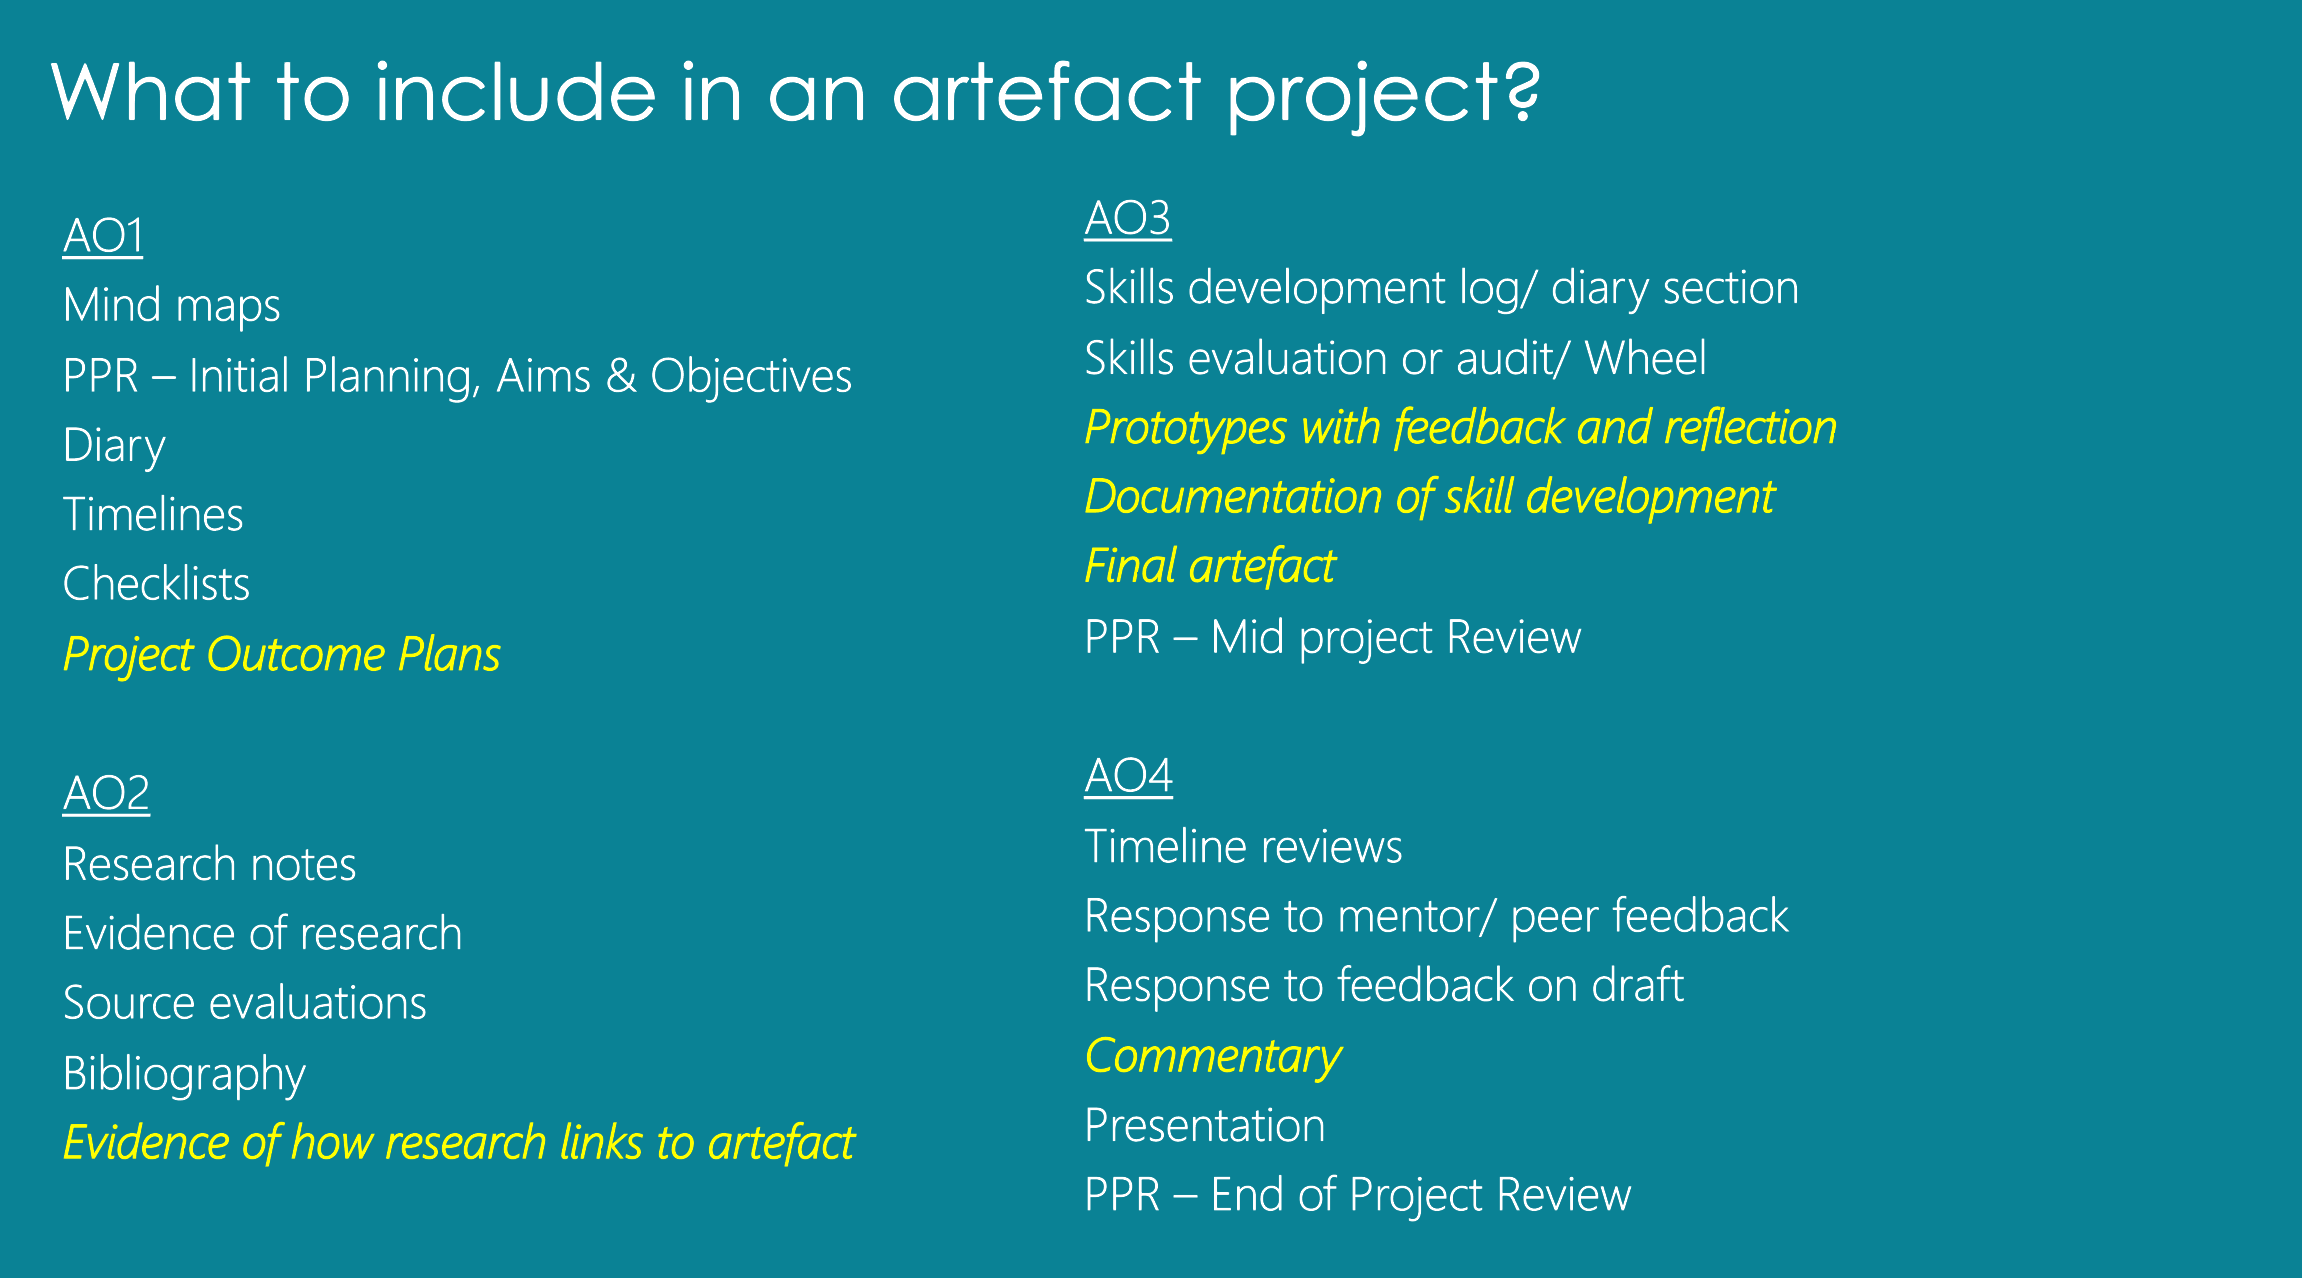
\includegraphics[width=0.8\textwidth]{Diary/22_WC_17-3-25/media/epqCriteria.png}
    \caption{A reminder of the critera i must hit during the EPQ project}
\end{figure}

Aside from EPQ day I spent some other time fixing errors in my code that I had noticed when demonstrating my project to family an friends

I also had the opportunity to present my work so far to a family member who is a senior figure at Microsoft and has previously had oversight over the note taking tools they offer. His feedback was certainly invaluable and he also pointed me to the Imagine Cup, a competition for students in colleges which I hope to partake in next year to further develop the skills I have been learning during this project. 


\subsection*{Power of Three:}
\textbf{This week's Tasks laid out per day}

\begin{tabularx}{\textwidth}{
  >{\raggedright\arraybackslash}X  % First column expands
  >{\centering\arraybackslash}p{1.5cm}  % Middle column has fixed width
  >{\raggedright\arraybackslash}X  % Third column expands
}
\toprule
\textbf{Goal} & \textbf{Achieved?} & \textbf{Notes} \\
\midrule


\rowcolor{gray!10}
\multicolumn{3}{l}{\textbf{Monday - Wednesday}} \\
Ability to visually make connections between notes  & \ding{51} & \\
Ensure new connections are saved to backend database & \ding{51} & \\
Note editor insert pdf  & \ding{55} & added to future list as will build within the whiteboard note type \\
When opening notes in a tab rename that tab to reflect the note name & \ding{51} & \\
Able to rename Notes and Tags in the graph view & \ding{51} & \\
Ensure all aspects of UI only show the most up to date names to avoid confusion & \ding{51} & \\
Make tab[0] be a refresh tab showing a spinner, call it whenever refreshing content & \ding{51} & \\
Fix tab filters so they only show content that is in current view scope & \ding{51} & \\

\rowcolor{gray!10}
\multicolumn{3}{l}{\textbf{Thursday}} \\
\nameref{planning:EPQDayPlan} & \ding{51} & Please open EPQ day plan page for more details\\

\bottomrule
\end{tabularx}


\subsection*{What went well?}
I have ticked many items of my to do list and feel confident in finishing my artifact fairly soon


\subsection*{What did I learn?}
I learnt about the benefits of waiting for a technology to become more developed and not just jumping on development with brand new, non documented technologies

\subsection*{What didn't quite go to plan?}
As outlined above I've rearranged my long-term plan to account for features I wasn't able to build this week


\subsection*{Plans for next week:}
continue artefact development